\section{Versuchsaufbau und Durchführung}
\label{sec:Versuchaufbau}

Der in diesem Experiment verwendete Versuchsaufbau ist in Abbildung \ref{fig:plot4} dargestellt. 

\begin{figure}
  \centering
  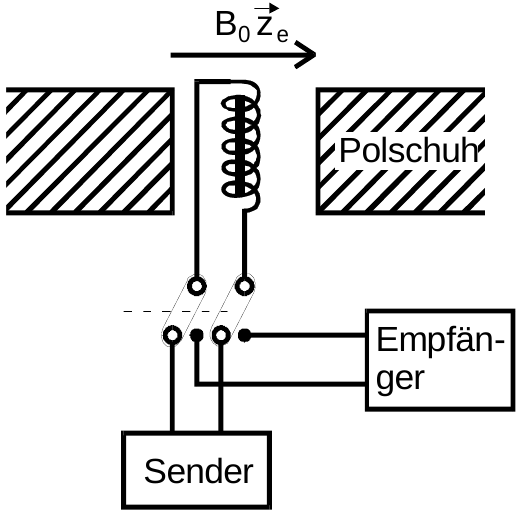
\includegraphics[width=0.40\textwidth]{ressources/Aufbau.png}
  \caption{Skizze des Messaufbaus.}
  \label{fig:plot4}
\end{figure}


Der Elektromagnet erzeugt das konstante Magnetfeld in $z$-Richtung. Im annähernd homogenen Magentfeld befindet sich die Probe in Mitten einer Spule. Durch ein HF-Signal ensteht somit ein Wechselfeld in $x$-Richtung. Als Empfängergerät wird ein Oszilloskop verwendet, welches die beiden transversalen Kompenenten der Magnetisierung anzeigt.

Zu Beginn erfolgt die Justage. Dafür wird eine Kupfersulfat-Lösung verwendet, welches eine deutlich kürzere Relaxationszeit aufweißt, sodass der Einstellvorgang beschleunigt werden kann. Es werden die folgenden Parameter verwendet:
\begin{align}
	\text{A-Puls}&=\SI{2}{\micro\second}\\
	\text{Wiederholzeit} \;\;P &= \SI{0.5}{\second}\\
	\text{Frequenz}\;\; \nu &=\SI{21.7}{\mega\hertz}
\end{align}
Ausgehend von diesen Startparametern wird die Amplitude des FID (Free Induction Decay) mit Hilfe der Frequenz, Phase und Pulslänge iterativ maximiert. Anschließend wird die Probe gegen destillierstes Wasser ausgetauscht und die Einstellungen überprüft und wenn nötig nochmals variiert. 

In der ersten Messungen wird die Zeitkonstante $T_1$ ermittelt, indem ein $\Delta t_{180}$-Puls und dann ein $\Delta t_{90}$-Puls erzeugt wird. Die Amplitude des entstehenden Echos wird am Oszilloskop abgelesen. Dieser Vorgang wird für verschiedene Impulsabstände $\tau$ wiederholt.

Für die Bestimmung der Zeitkonstante $T_2$, wird die Meiboom-Gill-Methode genutzt. Dafür wird zum einen die Pulsreihenfolge verändert und zum anderen die Anzahl der Pulse $B=100$ gewählt. Der auf dem Oszilloskop dargestellte exponentielle Abfall der Amplitude wird auf einem USB-Stick gespeichert. 

Zur analyse der Diffusionskontante wird der $z$-Gradient maximiert, sodass eine maximale Inhomogenität erreicht wird. Mit dem Spin-Echo-Verfahren wird dann ein Echo erzeugt ($B=1$) und dessen Amplitude erneut am Oszilloskop abgelesen. Aufgrund der verstärkten Diffusion kann das Echo nur für $\tau<\SI{30}{\milli\second}$ untersucht werden. Zudem wird ein Abbild der Messung erneut auf einem USB-Stick gepeichert, um die Halbwertsbreite des Echos zu ermitteln.

Zuletzt ist die Viskosität von Wasser mit Hilfe eines Viskosimeter bei Raumtemperatur zu bestimmen. Dafür wird der Zeitraum gemessen indem eine bestimmte Menge Wasser eine markierte Strecke im Viskosimeter zurücklegt.